\documentclass[11pt]{article}

\usepackage[margin=1in]{geometry}
\usepackage[T1]{fontenc}
\usepackage[utf8]{inputenc}
\usepackage[english]{babel}
\usepackage{lmodern}
\usepackage{microtype}
\usepackage{amsmath}
\usepackage{amssymb}
\usepackage{tabularx}
\usepackage{hyperref}
\usepackage{xcolor}
\usepackage{booktabs}
\usepackage{longtable}
\usepackage{array}
\usepackage{enumitem}
\usepackage{graphicx}
\usepackage{listings}
\usepackage{tikz}
\usetikzlibrary{arrows.meta, positioning, shapes.geometric, fit, calc, backgrounds}

\hypersetup{
  colorlinks=true,
  linkcolor=blue!50!black,
  urlcolor=blue!50!black,
  citecolor=blue!50!black,
  pdftitle={Technical Description of the ML2 Final Project},
  pdfauthor={ml2_final_project}
}

\definecolor{codebg}{RGB}{247,247,247}
\definecolor{codeframe}{RGB}{220,220,220}

\lstdefinestyle{projectstyle}{
  basicstyle=\ttfamily\small,
  backgroundcolor=\color{codebg},
  frame=single,
  rulecolor=\color{codeframe},
  breaklines=true,
  columns=fullflexible,
  keepspaces=true,
  showstringspaces=false,
  tabsize=2
}

\lstset{style=projectstyle}

\newcommand{\pathtt}[1]{\texttt{#1}}

\title{Technical Description of the Project Architecture, Data Pipeline, and Training Workflow\\ \large (Updated for End-to-End Architecture)}
\author{ml2\_final\_project}
\date{\today}

\begin{document}

\maketitle

\begin{abstract}
This document explains the project at the level a new reader needs first: how the repository is organized, how the data moves from raw corpora to processed tensors, how the training code is split into reusable modules, and how the experiment folders are produced. The architecture has been updated to an End-to-End (E2E) framework utilizing a Global Style Token (GST) and Normalizing Flows to allow real-time cross-lingual voice conversion.
\end{abstract}

\tableofcontents
\newpage

\section{Proposal}
The goal of this project is to build an end-to-end, real-time model for cross-lingual voice conversion. The model will be trained with the following datasets: LibriSpeech-PT, TTS Portuguese Corpus, and LibriSpeech-EN. It leverages pre-trained foundational models (XLM-RoBERTa for text and HuBERT for audio) combined with a Global Style Token (GST) to disentangle language content from speaker prosody.

\section{Repository Overview}

The repository is divided into a few clear responsibilities: raw data storage, preprocessing, reusable code, experiment outputs, and documentation.

\subsection{High-Level Directory Tree}

\begin{lstlisting}
ml2_final_project/
|-- data/
|   |-- raw/
|   |   |-- libriSpeech-pt/
|   |   `-- tts-portuguese-Corpora/
|   |-- processed/
|   |   |-- libriSpeech-pt/
|   |   |   |-- train/
|   |   |   |   `-- librispeech_mels_metadata.csv
|   |   |   `-- test/
|   |   |       `-- librispeech_mels_metadata.csv
|   |   `-- tts_portuguese/
|   |       `-- mels_metadata.csv
|   |-- interim/
|   `-- external/
|-- scripts/
|   |-- download_datasets/
|   `-- preprocess/
|       |-- preprocess_libriSpeech-pt.py
|       `-- preprocess_mels_tts_portuguese.py
|-- src/
|   |-- data/
|   |   `-- first_step_data_loaders/
|   |       `-- datasets.py
|   |-- models/
|   |   |-- PosteriorEncoder.py
|   |   |-- GST.py
|   |   |-- TextEncoder.py
|   |   |-- NormalizingFlow.py
|   |   `-- HiFi-GAN.py
|   `-- training/
|       `-- train_first_step/
|           |-- train.py
|           |-- model_loader.py
|           |-- losses.py
|           |-- train_utils.py
|           |-- text_processing.py
|           |-- configs.py
|           |-- run_training.py
|           `-- checkpoint_utils.py
|-- experiments/
|   `-- step_1/
|       `-- attempt_<timestamp>/
`-- docs/
\end{lstlisting}

\subsection{What Each Major Folder Means}

\begin{longtable}{>{\raggedright\arraybackslash}p{0.23\textwidth} >{\raggedright\arraybackslash}p{0.71\textwidth}}
\toprule
\textbf{Folder} & \textbf{Role in the project} \\
\midrule
\pathtt{data/raw} & Original corpora exactly as downloaded. Nothing here should depend on a model version or a feature extraction recipe. \\
\pathtt{data/processed} & Processed artifacts such as \pathtt{.pt} files and metadata CSV manifests used by the dataset layer. \\
\pathtt{data/interim} & Temporary intermediate outputs or scratch files. \\
\pathtt{scripts/preprocess} & Reproducible preprocessing scripts that convert raw audio into filtered, normalized, indexed training samples. \\
\pathtt{src/data} & Dataset wrappers and batching helpers that turn manifests into PyTorch objects. \\
\pathtt{src/models} & Reusable neural network components (GST, Encoders, Flows, Vocoder). \\
\pathtt{src/training} & Training orchestration, losses, configuration presets, checkpointing, and experiment utilities. \\
\pathtt{experiments} & Timestamped or named experiment outputs. Each run keeps its config, checkpoints, logs, and TensorBoard data together. \\
\pathtt{docs} & Technical descriptions, reports, and the LaTeX sources. \\
\bottomrule
\end{longtable}

\section{End-to-End Data Flow}

The project follows a simple lifecycle:

\begin{enumerate}[leftmargin=1.5em]
  \item Download raw corpora into \pathtt{data/raw}.
  \item Preprocess audio and transcripts into standardized tensors.
  \item Save per-utterance artifacts and metadata manifests in \pathtt{data/processed}.
  \item Load the processed manifests with the dataset classes in \pathtt{src/data}.
  \item Build the training experiment from the modules in \pathtt{src/training}.
  \item Save checkpoints, logs, and plots under \pathtt{experiments/step\_1}.
\end{enumerate}

\subsection{Data Pipeline Diagram}

\begin{center}
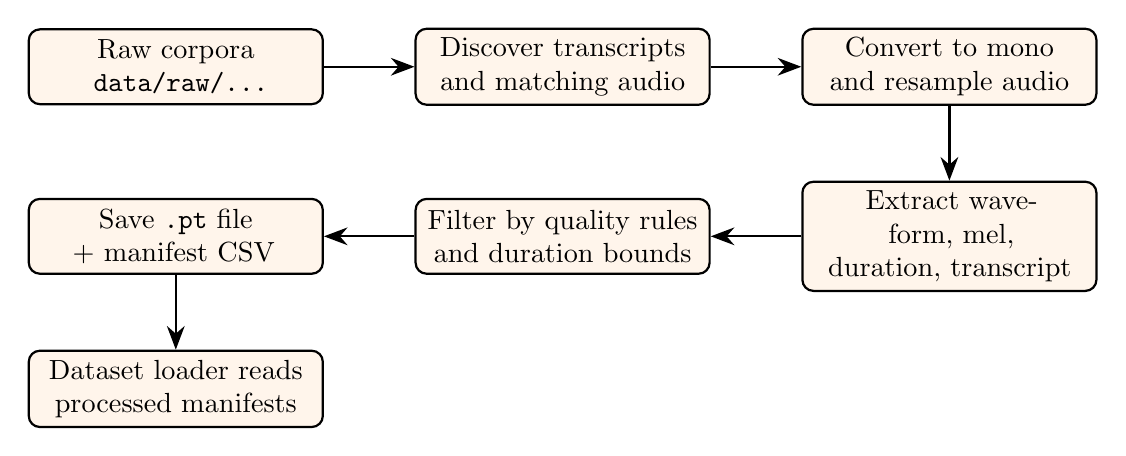
\begin{tikzpicture}[
  node distance=0.95cm and 1.15cm,
  block/.style={draw, rounded corners, thick, align=center, minimum height=0.95cm, text width=3.5cm, fill=orange!8},
  arrow/.style={-{Stealth[length=3mm]}, thick}
]
\node[block] (raw) {Raw corpora\\\pathtt{data/raw/...}};
\node[block, right=of raw] (discover) {Discover transcripts\\and matching audio};
\node[block, right=of discover] (normalize) {Convert to mono\\and resample audio};
\node[block, below=of normalize] (extract) {Extract waveform, mel,\\duration, transcript};
\node[block, left=of extract] (filter) {Filter by quality rules\\and duration bounds};
\node[block, left=of filter] (save) {Save \pathtt{.pt} file\\+ manifest CSV};
\node[block, below=of save] (load) {Dataset loader reads\\processed manifests};

\draw[arrow] (raw) -- (discover);
\draw[arrow] (discover) -- (normalize);
\draw[arrow] (normalize) -- (extract);
\draw[arrow] (extract) -- (filter);
\draw[arrow] (filter) -- (save);
\draw[arrow] (save) -- (load);
\end{tikzpicture}
\end{center}

\section{How Data Should Be Organized}

\subsection{Raw Data Layout}
Place each corpus in its own directory under \pathtt{data/raw}. A practical example is:

\begin{lstlisting}
data/raw/
|-- libriSpeech-pt/
|   `-- mls_portuguese_opus/
|       |-- train/
|       |-- dev/
|       `-- test/
`-- tts-portuguese-Corpora/
    `-- TTS-Portuguese-Corpus/
        |-- audio/
        |-- text/
        `-- metadata/
\end{lstlisting}

In this structure, the preprocessing scripts can discover transcripts and audio without mixing source corpora or overwriting the downloaded archives.

\subsection{Processed Data Layout}
The processed area mirrors the dataset identity and the split. The dataset classes use manifests directly. A representative layout is:

\begin{lstlisting}
data/processed/
|-- libriSpeech-pt/
|   |-- train/
|   |   |-- pt_000123.pt
|   |   |-- pt_000124.pt
|   |   `-- librispeech_mels_metadata.csv
|   `-- test/
|       |-- pt_010001.pt
|       `-- librispeech_mels_metadata.csv
`-- tts_portuguese/
    |-- ttsp_000045.pt
    `-- mels_metadata.csv
\end{lstlisting}

Example manifest row:

\begin{lstlisting}[language=]
utt_id,text,duration,mel_path,audio_path,source
pt_000123,ola mundo,2.83,data/processed/libriSpeech-pt/train/pt_000123.pt,data/raw/libriSpeech-pt/.../pt_000123.flac,libriSpeech-pt
\end{lstlisting}

\subsection{What Goes Into a \pathtt{.pt} File}
Each serialized sample should keep everything needed to train:
\begin{itemize}[leftmargin=1.5em]
  \item \pathtt{waveform}: the resampled mono waveform tensor (22050Hz).
  \item \pathtt{mel}: the log-mel spectrogram tensor, with 80 mel bins.
  \item \pathtt{sr}: the sample rate used by preprocessing.
  \item \pathtt{duration}: utterance duration in seconds.
  \item \pathtt{text}: the transcript text after normalization.
  \item \pathtt{utt\_id}: the unique utterance identifier.
\end{itemize}

\subsection{Example Sample Payload}
One saved example may contain the following keys and values:

\begin{lstlisting}[language=]
{
  "waveform": Tensor([1, T]),
  "mel": Tensor([80, M]),
  "sr": 22050,
  "duration": 2.83,
  "text": "ola mundo",
  "utt_id": "pt_000123",
  "audio_path": "data/raw/libriSpeech-pt/.../pt_000123.flac"
}
\end{lstlisting}

\textbf{Note on Mel-Spectrograms:} Since the original `.pt` files contain mels that are not natively in the optimal latent space for HiFi-GAN, a \textit{Posterior Encoder} is introduced in the architecture to project these 80-bin mels into the correct latent space $z$.

\subsection{How the Pipeline Fits Together}
The full pipeline works as a sequence of reusable steps:

\begin{enumerate}[leftmargin=1.5em]
  \item Raw corpora are downloaded into \pathtt{data/raw}.
  \item The preprocessing scripts discover audio files and transcripts.
  \item Audio is normalized, resampled, and converted into mel tensors.
  \item Each utterance is stored as one \pathtt{.pt} file plus a manifest row.
  \item The dataset loaders read the manifests and reconstruct training examples.
  \item Training code consumes the examples and writes experiment outputs under \pathtt{experiments/step\_1}.
\end{enumerate}

\subsection{Example Commands and How to Use Them}
Run these commands from the repository root. The backslash at the end of a line means the command continues on the next line, which keeps long commands readable.

\begin{lstlisting}[language=bash]
# Preprocess LibriSpeech-PT into processed tensors and a manifest
python scripts/preprocess/preprocess_libriSpeech-pt.py \
  --input-dir data/raw/libriSpeech-pt/mls_portuguese_opus \
  --out-dir data/processed/libriSpeech-pt/train \
  --target-sr 22050 \
  --n-mels 80 \
  --n-fft 1024 \
  --hop-length 256 \
  --win-length 1024 \
  --min-duration 1.0 \
  --max-duration 10.0

# Preprocess the TTS Portuguese corpus
python scripts/preprocess/preprocess_mels_tts_portuguese.py \
  --input-dir data/raw/tts-portuguese-Corpora/TTS-Portuguese-Corpus \
  --out-dir data/processed/tts_portuguese \
  --target-sr 22050

# Start a quick training smoke test
python src/training/train_first_step/run_training.py quick_test

# Start a larger preset
python src/training/train_first_step/run_training.py balanced

# Launch a custom training run
python src/training/train_first_step/train.py \
  --num-epochs 100 \
  --batch-size 32 \
  --learning-rate 1e-3 \
  --weight-reconstruction 1.0 \
  --weight-diversity 0.5 \
  --num-workers 4 \
  --experiment-name cross_lingual_training
\end{lstlisting}

Use the preprocessing commands first so the processed directories exist before training starts. Use the preset commands when you want a reproducible configuration quickly, and use the custom command when you need to change the batch size, learning rate, or loss weights.

\subsection{How to Read the Flags}
\begin{itemize}[leftmargin=1.5em]
  \item \pathtt{--input-dir}: points to the raw corpus folder.
  \item \pathtt{--out-dir}: tells the script where to write processed files.
  \item \pathtt{--target-sr}: sets the sample rate used during preprocessing.
  \item \pathtt{--num-epochs}: controls how many epochs the trainer will run.
  \item \pathtt{--batch-size}: sets the number of samples per optimization step.
  \item \pathtt{--learning-rate}: sets the optimizer step size.
  \item \pathtt{--weight-reconstruction} and \pathtt{--weight-diversity}: control how the loss terms are balanced.
  \item \pathtt{--experiment-name}: names the run directory under \pathtt{experiments/step\_1}.
\end{itemize}

\section{System Architecture: Train Structure}

The updated architecture replaces the cascaded Cross-Attention approach with an End-to-End (E2E) structure based on VITS principles. It utilizes a Posterior Encoder to map the training Mel-spectrograms into a unified latent space $z$, which the HiFi-GAN Vocoder is optimized to decode. Simultaneously, a Global Style Token (GST) extracts prosody and injects it into a Normalizing Flow, mapping the Text representations to the same latent space $z$.

\subsection{Pipeline Diagram}

\begin{center}
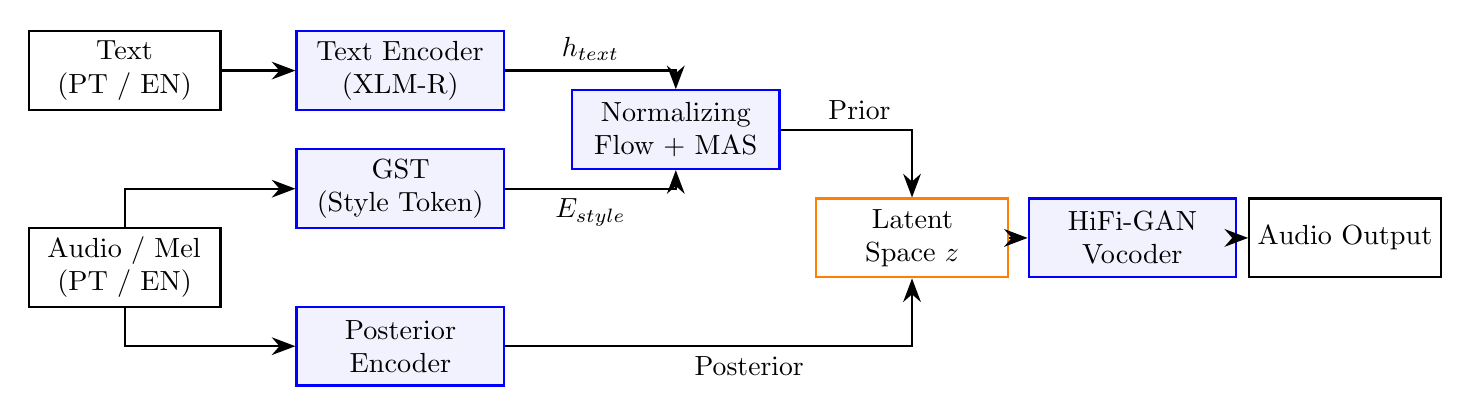
\begin{tikzpicture}[
  block/.style={draw, rectangle, thick, minimum height=1cm, minimum width=2.2cm, align=center, text width=2.2cm},
  model/.style={draw, rectangle, thick, fill=blue!5, draw=blue, minimum height=1cm, minimum width=2.2cm, align=center, text width=2.4cm},
  arrow/.style={-{Stealth[length=3mm]}, thick}
]

% Level 1: Text
\node[block] (text) at (0, 0) {Text\\(PT / EN)};
\node[model] (textenc) at (3.5, 0) {Text Encoder\\(XLM-R)};
\draw[arrow] (text) -- (textenc);

% Level 2 & 3: Audio / GST / Posterior
\node[block] (audio) at (0, -2.5) {Audio / Mel\\(PT / EN)};
\node[model] (gst) at (3.5, -1.5) {GST\\(Style Token)};
\node[model] (postenc) at (3.5, -3.5) {Posterior\\Encoder};
\draw[arrow] (audio) |- (gst);
\draw[arrow] (audio) |- (postenc);

% Level 1.5: Flow (Centered between Text and GST)
\node[model] (flow) at (7, -0.75) {Normalizing Flow + MAS};
\draw[arrow] (textenc.east) -| node[pos=0.25, above] {$h_{text}$} (flow.north);
\draw[arrow] (gst.east) -| node[pos=0.25, below] {$E_{style}$} (flow.south);

% Level 2.5: Latent space (Centered between Flow and Posterior)
\node[block, draw=orange] (latent) at (10, -2.125) {Latent\\Space $z$};
\draw[arrow] (flow.east) -| node[pos=0.3, above] {Prior} (latent.north);
\draw[arrow] (postenc.east) -| node[pos=0.3, below] {Posterior} (latent.south);

% Level 2.5: Vocoder & Output
\node[model] (hifigan) at (12.8, -2.125) {HiFi-GAN\\Vocoder};
\node[block] (out) at (15.5, -2.125) {Audio Output};
\draw[arrow] (latent) -- (hifigan);
\draw[arrow] (hifigan) -- (out);

\end{tikzpicture}
\end{center}

\begin{sloppypar}
During training, the \pathtt{Posterior Encoder} turns the processed 80-bin mel tensors into latent space $z$.
The \pathtt{GST} computes a global style embedding.
The \pathtt{Normalizing Flow} aligns text with audio frames.
The vocoder is trained on the extracted $z$.
\end{sloppypar}

\subsection{Architecture Specifications and Dimensions}

To successfully implement this E2E architecture, the modules must adhere to specific tensor dimensions and layer configurations.

\begin{itemize}[leftmargin=1.5em]
    \item \textbf{Text Encoder (XLM-RoBERTa Base):}
    \begin{itemize}
        \item \textbf{Input:} Tokenized text sequence.
        \item \textbf{Architecture:} 12 Transformer layers, 12 attention heads.
        \item \textbf{Output ($h_{text}$):} Sequence of embeddings with dimension $\mathbb{R}^{T_{text} \times 768}$.
    \end{itemize}
    \item \textbf{Global Style Token (GST):}
    \begin{itemize}
        \item \textbf{Input:} 80-bin Mel-spectrogram of the reference audio.
        \item \textbf{Architecture:} A 2D Convolutional reference encoder (6 layers) followed by Multi-Head Attention over a bank of learnable style tokens.
        \item \textbf{Output ($E_{style}$):} A fixed-length global style embedding with dimension $\mathbb{R}^{256}$.
    \end{itemize}
    \item \textbf{Posterior Encoder:}
    \begin{itemize}
        \item \textbf{Input:} 80-bin target Mel-spectrogram.
        \item \textbf{Architecture:} 16 layers of non-causal WaveNet residual blocks with dilation factors (e.g., 1, 2, 4, 8...).
        \item \textbf{Output ($z$):} Latent acoustic representation with dimension $\mathbb{R}^{T_{audio} \times 192}$.
    \end{itemize}
    \item \textbf{Normalizing Flow:}
    \begin{itemize}
        \item \textbf{Input:} Projected text embeddings aligned via MAS, conditioned globally on $E_{style}$.
        \item \textbf{Architecture:} 4 to 6 Affine Coupling Layers. Each coupling layer uses 4 WaveNet residual blocks with hidden dimension 192.
        \item \textbf{Output:} Maps the prior distribution to the posterior latent space $\mathbb{R}^{T_{audio} \times 192}$.
    \end{itemize}
    \item \textbf{HiFi-GAN Vocoder:}
    \begin{itemize}
        \item \textbf{Input:} Latent vector $z \in \mathbb{R}^{T_{audio} \times 192}$ (projected internally from 192 to the initial upsampling dimension, e.g., 512).
        \item \textbf{Architecture:} 4 Transposed Convolutions for upsampling. Suggested upsampling rates $k_u = [8, 8, 2, 2]$ for 22050 Hz. Multi-Receptive Field Fusion (MRF) modules added in parallel.
        \item \textbf{Output:} High-fidelity 1D waveform.
    \end{itemize}
\end{itemize}


\section{Loss Functions}

To ensure high-fidelity audio, prosody transfer, and stable training across languages, the loss objective incorporates Adversarial Learning, Contrastive Learning, and Variational bounds. The complete objective is:

\[
\mathcal{L}_{\text{total}} = \mathcal{L}_{\text{Recon}} + \lambda_{\text{KL}} \mathcal{L}_{\text{KL}} + \lambda_{\text{InfoNCE}} \mathcal{L}_{\text{InfoNCE}} + \mathcal{L}_{\text{Adv}}(G) + \mathcal{L}_{\text{FM}}
\]

\textbf{Mathematical Specifications:}
\begin{enumerate}[leftmargin=1.5em]
    \item \textbf{Mel Reconstruction Loss ($\mathcal{L}_{\text{Recon}}$):} Stabilizes the generator early on. Computed between the ground truth mel and the mel extracted from the HiFi-GAN output.
    \[
    \mathcal{L}_{\text{Recon}} = \| \text{Mel}_{\text{target}} - \text{Mel}(G(z)) \|_1
    \]

    \item \textbf{Kullback-Leibler Divergence ($\mathcal{L}_{\text{KL}}$):} Forces the Normalizing Flow's prior distribution $p(z | c_{\text{text}}, E_{\text{style}})$ to match the Posterior Encoder's output $q(z | \text{Mel}_{\text{target}})$.
    \[
    \mathcal{L}_{\text{KL}} = \int q(z | \text{Mel}) \log \frac{q(z | \text{Mel})}{p(z | c_{\text{text}}, E_{\text{style}})} \,dz
    \]

    \item \textbf{Contrastive Style Loss ($\mathcal{L}_{\text{InfoNCE}}$):} Enforces prosody and emotional consistency. It maximizes the cosine similarity between the GST token of the input audio ($s_i$) and the GST token extracted from the generated audio ($\hat{s}_i$), while pushing away negative samples in the batch.
    \[
    \mathcal{L}_{\text{InfoNCE}} = - \frac{1}{N} \sum_{i=1}^{N} \log \frac{\exp(\text{sim}(s_i, \hat{s}_i) / \tau)}{\sum_{j=1}^{N} \exp(\text{sim}(s_i, s_j) / \tau)}
    \]

    \item \textbf{Adversarial \& Feature Matching Loss ($\mathcal{L}_{\text{Adv}}, \mathcal{L}_{\text{FM}}$):} Standard HiFi-GAN Least-Squares losses evaluated via Multi-Period and Multi-Scale Discriminators (MPD/MSD).
    \[
    \mathcal{L}_{\text{Adv}}(G) = \mathbb{E}_z \left[ (D(G(z)) - 1)^2 \right]
    \]
    \[
    \mathcal{L}_{\text{FM}} = \mathbb{E}_{x, z} \left[ \sum_{l=1}^{L} \frac{1}{N_l} \| D^{(l)}(x) - D^{(l)}(G(z)) \|_1 \right]
    \]
\end{enumerate}

\section{Inference Workflow}

\begin{sloppypar}
During inference, we bypass the Posterior Encoder entirely.
We extract the Style Token from the source Portuguese audio via the GST.
We encode the English text and combine it with the Style Token.
The Normalizing Flow runs in reverse to generate the latent variable $z'$.
The Vocoder synthesizes the final English audio.
\end{sloppypar}

\subsection{Inference Architecture Diagram}

\begin{center}
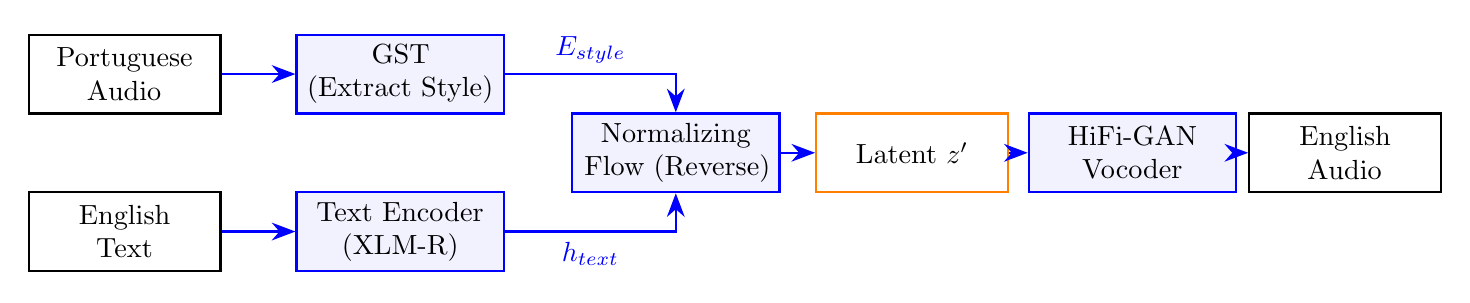
\begin{tikzpicture}[
  block/.style={draw, rectangle, thick, minimum height=1cm, minimum width=2.2cm, align=center, text width=2.2cm},
  model/.style={draw, rectangle, thick, fill=blue!5, draw=blue, minimum height=1cm, minimum width=2.2cm, align=center, text width=2.4cm},
  arrow/.style={-{Stealth[length=3mm]}, thick, blue}
]

\node[block] (audio_pt) at (0, 0) {Portuguese\\Audio};
\node[model] (gst) at (3.5, 0) {GST\\(Extract Style)};
\draw[arrow] (audio_pt) -- (gst);

\node[block] (text_en) at (0, -2) {English\\Text};
\node[model] (textenc) at (3.5, -2) {Text Encoder\\(XLM-R)};
\draw[arrow] (text_en) -- (textenc);

\node[model] (flow) at (7, -1) {Normalizing Flow (Reverse)};
\draw[arrow] (gst.east) -| node[pos=0.25, above] {$E_{style}$} (flow.north);
\draw[arrow] (textenc.east) -| node[pos=0.25, below] {$h_{text}$} (flow.south);

\node[block, draw=orange, text=black] (latent) at (10, -1) {Latent $z'$};
\draw[arrow] (flow) -- (latent);

\node[model] (hifigan) at (12.8, -1) {HiFi-GAN\\Vocoder};
\node[block, text=black] (audio_en) at (15.5, -1) {English\\Audio};
\draw[arrow] (latent) -- (hifigan);
\draw[arrow] (hifigan) -- (audio_en);

\end{tikzpicture}
\end{center}

\section{Training Code Organization in \pathtt{src}}

The training pipeline is split into small modules so that each concern has one main place in the codebase.

\subsection{Module Map}

\begin{longtable}{>{\raggedright\arraybackslash}p{0.25\textwidth} >{\raggedright\arraybackslash}p{0.69\textwidth}}
\toprule
\textbf{Module} & \textbf{What it does} \\
\midrule
\pathtt{train.py} & Main training entry point. Builds datasets and runs training. \\
\pathtt{model\_loader.py} & Loads the pre-trained components and assembles the network. \\
\pathtt{losses.py} & Implements KL, InfoNCE, and adversarial losses. \\
\pathtt{train\_utils.py} & Contains epoch loops, checkpoints, and alignment helpers. \\
\bottomrule
\end{longtable}

\section{How to Run Experiments \& Training Phases}

Because the architecture utilizes massive pre-trained models, training must be phased to prevent catastrophic forgetting.

\subsection{Phase 1: Flow \& Alignment (Epochs 0 - 100)}
\begin{itemize}[leftmargin=1.5em]
    \item \textbf{Action:} Freeze XLM-R and HiFi-GAN Vocoder. Train only the Posterior Encoder, GST, and Normalizing Flows.
    \item \textbf{Goal:} Find the Monotonic Alignment (MAS) and optimize $\mathcal{L}_{\text{KL}}$.
    \item \textbf{Learning Rate:} $2 \times 10^{-4}$ (AdamW).
\end{itemize}

\subsection{Phase 2: Acoustic Fine-Tuning (Epochs 101 - 250)}
\begin{itemize}[leftmargin=1.5em]
    \item \textbf{Action:} Unfreeze HiFi-GAN generators and discriminators.
    \item \textbf{Goal:} Optimize $\mathcal{L}_{\text{Adv}}$, $\mathcal{L}_{\text{FM}}$, and $\mathcal{L}_{\text{Recon}}$ for high-fidelity audio synthesis. Incorporate InfoNCE for prosody.
    \item \textbf{Learning Rate:} $1 \times 10^{-4}$.
\end{itemize}

\subsection{Phase 3: End-to-End Joint Training (Epochs 251 - 500)}
\begin{itemize}[leftmargin=1.5em]
    \item \textbf{Action:} Unfreeze the last 4 layers of XLM-R. Train the entire pipeline end-to-end.
    \item \textbf{Goal:} Minimize $\mathcal{L}_{\text{total}}$.
    \item \textbf{Learning Rate:} Drop foundational model LR to $1 \times 10^{-5}$, keep Flow/Vocoder at $1 \times 10^{-4}$.
\end{itemize}

\subsection{Example Commands}

\begin{lstlisting}[language=bash]
# Phase 1: Warmup & Flow Alignment
python src/training/train_first_step/train.py \
  --num-epochs 100 \
  --batch-size 32 \
  --learning-rate 2e-4 \
  --freeze-text-encoder \
  --freeze-vocoder \
  --experiment-name phase1_flow_alignment

# Phase 3: E2E Joint Training
python src/training/train_first_step/train.py \
  --resume-from checkpoints/phase2_latest.pt \
  --num-epochs 250 \
  --batch-size 16 \
  --learning-rate-base 1e-5 \
  --learning-rate-flow 1e-4 \
  --lambda-kl 1.0 \
  --lambda-infonce 0.1 \
  --experiment-name phase3_e2e_finetune
\end{lstlisting}

\section{Summary}

The E2E architecture fundamentally resolves the bottleneck of translating Mel-spectrograms directly. By treating both languages and prosody as separate embeddings in a unified Normalizing Flow, the model achieves real-time inference with a single forward pass, heavily capitalizing on foundational weights (XLM-R) and high-fidelity vocoders (HiFi-GAN).

\end{document}